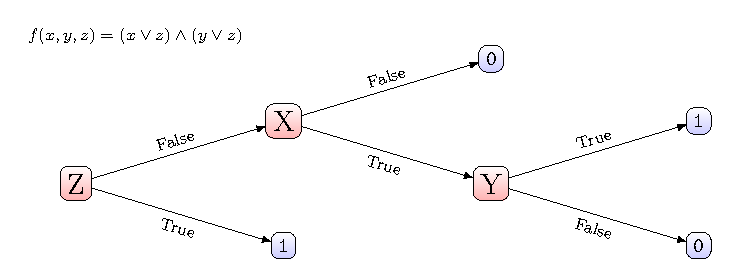
\includegraphics{decision_tree.pdf}
\begin{description}
	\item[$\bullet$] The variable $z$ was chosen as the first node, because if $z = 1$, then $f(x,y,z) = 1$.
	\item[$\bullet$] If $z$ is False, the function could lead to both $x$ or $y$, giving the commutative property. In case $x$ is False, the output will be 0.
	\item[$\bullet$] If $x$ is True, the last variable to be analyzed is $y$. Similarly to $x$, $y$ needs to be True, in order to the output equals 1.
\end{description}

